\section{Numerical Experiments}\label{sec:crqi:experiments}
The purpose of this section is twofold. First, we study various
numerical examples to understand the behaviour of CRQI and demonstrate
the good properties we already mentioned at the beginning of the
chapter.  Second, we illustrate the erratic behaviour of classic RQI
that we mentioned several times before. This is not done separately
but by running the same experiments for both methods and comparing the
results throughout. All experiments were executed in Matlab~9~\cite{MATLAB}. The criterion for convergence is
$\norm*{\vec{r}^{(k)}} = \norm*{\mat{A}\vec{x}^{(k)} - \mu^{(k)}
  \vec{x}^{(k)}} < 10^{-9}$. The source codes for both classic and
complex RQI can be found in Appendix~\ref{AppendixAlgorithms}. Note
that the methods are defined slightly differently from the Algorithms
given above. They both allow to explicitly set the initial shifts
$\mu^{(0)}$ and $\gamma^{(0)}$ to specific values whereas in
Algorithm~\ref{alg:rqi} and Algorithm~\ref{alg:crqi} the initial
shifts are always initialised to the Rayleigh Quotient of the initial
vector and the initial residual, respectively. This will become useful
when investigating how the initial shift influences the outcome of the
method.

All of the experiments were carried out for different matrices that
are common for assessing eigenvalue algorithms. In particular, they
have been used to evaluate shift-and-invert type algorithms and
algorithms related to classic RQI, see, \eg\cite{dax2003} and the
references therein. They are described below. Recall that we are
particularly interested in problems with closely spaced eigenvalues
and, except for the first example, all of the test matrices will lead
to such problems. Since in three of the test problems the spacing even
becomes closer the larger the matrix gets, we will also study the
algorithm's behaviour under increasing matrix size.

\paragraph{Random matrices}
These matrices are pseudo-randomly generated using the Matlab command
``sprandsym''. Apart from being sparse and symmetric, they have no
special structure or properties.

\paragraph{The matrix $[1,2,1]$} This matrix is a tridiagonal matrix
with all diagonal elements set to 2 and all off-diagonal elements set
to 1. The eigenvalues of this matrix are all distinct and their exact
values are known to be
\begin{equation*}
  \lambda_k = 4 \sin^2\left(\frac{\pi k}{2(n+1)} \right)\,,
\end{equation*}
where $n$ denotes the order (\ie the number of rows) of the
matrix~\cite[299--307]{wilkinson}. Thus, for every $n$, the
eigenvalues lie in the interval $[0,4]$ and so consequently their
spacing gets smaller the larger the matrix gets.

\paragraph{Wilkinson's matrix $\mat{W}^+$}
This tridiagonal matrix was extensively studied by Wilkinson
in~\cite{wilkinson}, hence its name. It is of order $n = 2p + 1$ for
some $p \in \N$. The $m$th diagonal entry is set to $\abs{p+1-m}$ and
all off-diagonal entries are set to 1. For instance, for $p=2$ this
yields the $5 \times 5$ matrix
\begin{equation*}
  \mat{W}^+_5 = 
  \begin{bmatrix}
    2 & 1 \\
    1 & 1 & 1 \\
    & 1 & 0 & 1 \\
    && 1 & 1 & 1 \\
    &&& 1 & 2
  \end{bmatrix}\,.
\end{equation*}
The spectrum consists of pairs of nearly, but not exactly, equal
eigenvalues. For example, the two largest eigenvalues of
$\mat{W}^+_{21}$ agree to 15 significant
decimals~\cite[300--309]{wilkinson}.

\paragraph{The Martin-Wilkinson matrix $\mat{MW}$}
If we denote by $a_{jk}$ the $k$th entry of the $j$th row of
$\mat{MW}$, the nonzero entries of this matrix are defined by
\begin{align*}
  a_{jj} &= 6 \quad &&\text{for } j = 2,\dotsc,n-1 \quad \text{but } a_{11} = a_{nn} = 5, \\
  a_{j,j-1} = a_{j-1,j} &= -4 \quad &&\text{for } j = 2,\dotsc,n, \\
  a_{j,j-2} = a_{j-2,j} &= 1 \quad &&\text{for } j = 2, \dotsc, n\,.
\end{align*}
The eigenvalues are known to be~\cite[39]{galligani}
\begin{equation*}
  \lambda_m = 16 \sin^4\left(\frac{m \pi}{2(n+1)} \right)
\end{equation*}
and thus, independent of $n$, the eigenvalues lie in the interval
$[0,16]$. Hence, the eigenvalues become increasingly close the larger
the size of the matrix.
% \footnote{We adopted the name \emph{Martin-Wilkkinson matrix}
% from~\cite{dax2003}. The author refers to a paper of Martin and
% Wilkinson where this matrix is used to }

\paragraph{The Laplace matrix $\mat{L}$}
This matrix arises, for instance, when discretising the Laplace
operator using a five-point stencil in the finite difference method
(see, for example,~\cite[270--272]{demmel}). Let $m$ be an integer and
define the $m \times m$ matrix
\begin{equation*}
  \mat{T} =
  \begin{bmatrix}
    4 & -1 \\
    -1 & 4 & -1 \\
    & \ddots & \ddots & \ddots \\
    && -1 & 4 & -1 \\
    &&& -1 & 4
  \end{bmatrix}\,.
\end{equation*}
The Laplace matrix is a block tridiagonal matrix of order $n = m^2$
defined as
\begin{equation*}
  \mat{L} =
  \begin{bmatrix}
    \mat{T} & -\mat{I} \\
    -\mat{I} & \mat{T} & -\mat{I} \\
    & \ddots & \ddots & \ddots \\
    && -\mat{I} & \mat{T} & -\mat{I} \\
    &&& -\mat{I} & \mat{T}
  \end{bmatrix}\,,
\end{equation*}
where $\mat{I}$ is the $m \times m$ identity matrix. Again, the
eigenvalues can be computed analytically and all lie in an interval
that is independent of the matrix's size; in this case they are all
contained in the interval $[0,8]$.

\bigskip%
Below we give some numerical examples that highlight different
behavioural aspects of the algorithm. Plots and/or tables that
illustrate our findings are given for each of the test matrices. They
are either included directly within the example or can be found in
Appendix~\ref{appendix:plots}. Those included in this section are the
ones we found most meaningful for the particular example.

Recall that we assume that a good approximation of the wanted
eigenvector is available. To simulate this, the full set of
eigenvectors is computed using built-in Matlab routines. These vectors
are then collected as columns of a matrix $\mat{V}$. Next, a weight
vector $\vec{w}$ of uniformly distributed numbers between $0$ and $1$
is created. One of the components is set to a higher value than the
others, e.\,g., $w_{50} = 10$ (in most examples the index of the
component was also chosen randomly). The initial vector is then set to
a weighted linear combination of the eigenvectors, \ie
$\vec{x}^{(0)} = \beta \mat{V} \vec{w}$, where $\beta$ has to be
chosen such that $\vec{x}^{(0)}$ is normalised. Now, $\vec{x}^{(0)}$
is a vector with a strong component in the direction of the target
eigenvector (in this case this would be $\vec{v}_{50}$) and random
(smaller) contributions in the directions of the other eigenvectors.

\begin{example}
  The first example demonstrates how difference choices for the
  imaginary shift $i\gamma^{(k)}$ affect the convergence speed. We run
  three different variants of CRQI:\@ The first uses
  $\gamma^{(k)} = \norm*{\vec{r}^{(k)}}$, which is the same as in
  Algorithm~\ref{alg:crqi} above. The second uses the square of the
  residual norm, the third approach is explained below. A plot of the
  residual norms against the iteration number for all three approaches
  together with the results using classic RQI\footnote{Classic RQI is
    merely included for speed comparison. In most of the examples it
    failed to converge to the correct eigenvalue.} is given in
  Figure~\ref{fig:residuals}.

\begin{figure}[htpb]
  \centering
  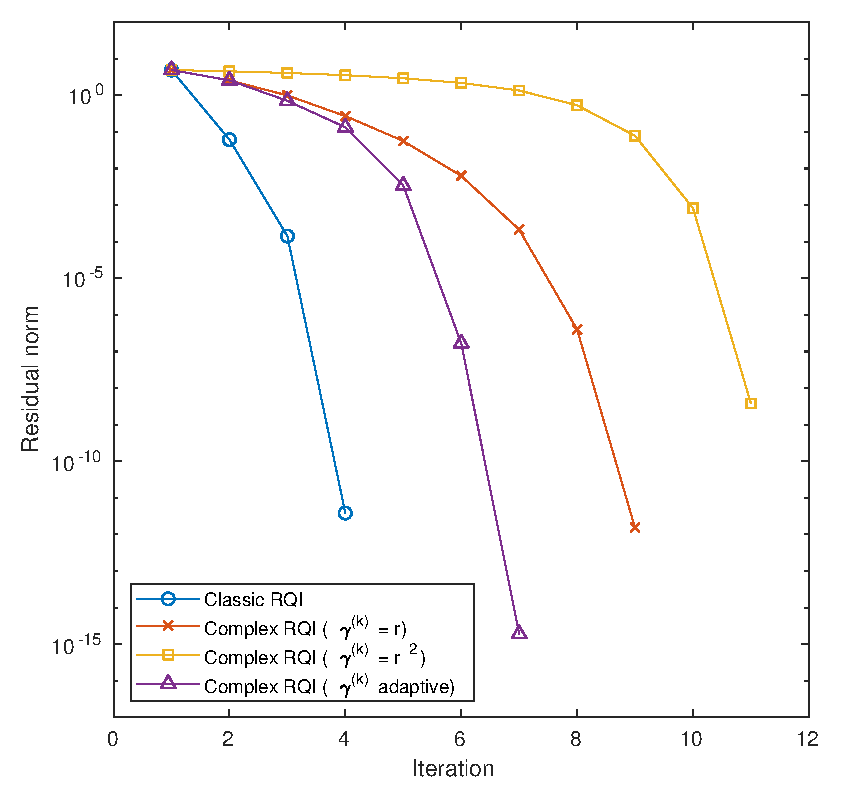
\includegraphics[width=0.65\textwidth]{Figures/crqi_residuals}
  \caption[Residuals for different choices of $\gamma^{(k)}$.]{Plot of
    residuals of Classic RQI, Complex RQI with
    $\gamma^{(k)} = \norm*{\vec{r}^{(k)}}$, Complex RQI with
    $\gamma^{(k)} = \norm*{\vec{r}^{(k)}}^2$ and Complex RQI with the
    imaginary shift chosen adaptively (see text) using a
    $1000\times 1000$ random matrix. The last variant seems to combine
    the advantages of the second and third alternatives.}%
  \label{fig:residuals}
\end{figure}

We observe that in the initial phase of the iteration, the second
variant (squared residual norm) seems to be slower than the
first. Although it might not be clearly observable in the figure,
further investigation of other examples suggested that during the
final steps of the iterations the second version was faster than the
first (see also Figures~\ref{fig:imag_shift:mat2}
to~\ref{fig:imag_shift:mat5} in the Appendix). Consequently, by
combining both approaches and thus changing the shift adaptively we
expect faster convergence. The results are also plotted in
Figure~\ref{fig:residuals} (labelled with ``$\gamma^{(k)}$ adaptive'')
and are in accordance with the expectation. In this particular case,
the shift was changed according to
\begin{equation*}
  \gamma^{(k)} =
  \begin{cases}
    \norm*{\vec{r}^{(k)}} & \text{ if } \norm*{\vec{r}^{(k)}} \ge 1\,, \\
    \norm*{\vec{r}^{(k)}}^2 & \text{ if } \norm*{\vec{r}^{(k)}} < 1\,.
  \end{cases}
\end{equation*}
In the following, when we speak of CRQI we mean CRQI performed with
this adaptive choice of imaginary shifts.

Running the same experiment but increasing the component of the
initial vector in the direction of the target eigenvector led to a
decrease of the number of additional steps required by CRQI; this
observation is analysed in more detail in Example~\ref{ex:its}. For
eigenvectors that were very close to the target sometimes both classic
RQI and complex RQI even finished within the same number of
iterations. Still, even in these cases, classic RQI often failed to
converge to the target eigenpair.

The plots also show that the convergence rate of CRQI (using the
adaptive choice of imaginary shifts) seems to be similar to that of
classic RQI and that it is the preasymptotic stage which comprises
more steps. Table~\ref{tab:ex1:convergence} shows the results of
classic RQI and CRQI, again using the adaptive choice of imaginary
shifts (for this example we slightly increased the residual tolerance
to $10^{-12}$). In the first four iterations of CRQI only one digit of
the eigenvalue approximation is correct. After this preasymptotic
stage, the method converges within three steps.
\end{example}

In the next examples we will examine how the initial vector and
initial (real) shift affect the results of RQI and CRQI. We have
already discussed the sometimes erratic behaviour of classic RQI. As
we will shortly see, a main problem of RQI is that convergence often
hardly depends on the initial vector but rather on the initial
shift. This is why especially for problems with closely spaced
eigenvalues RQI fails to compute the wanted eigenpair. CRQI seems to
be more robust to changes in the initial shift.

\begin{example}
  We start with an example where the algorithm was run many times with
  a fixed initial vector but varying initial shifts. To obtain the
  shifts we computed the spectrum of the matrix using built-in
  functions of Matlab and extracted 100 evenly-spaced values form the
  interval $[\lambda_{\text{min}} - 10, \lambda_{\text{max}} + 10]$,
  where $\lambda_{\text{min}}$ and $\lambda_{\text{max}}$ are the
  smallest and largest eigenvalue of $\mat{A}$, respectively (the
  numbers were slightly adapted for the other test matrices). The
  results using random matrices are plotted in Figure~\ref{fig:vary
    shift}. The initial vector was set to a weighted combination of
  the exact eigenvectors as described above. In the first two examples
  the contribution in the target direction was small while in the
  third example it was bigger. The last example shows the result using
  a vector that does not approximate any particular eigenvector.
  % The component in the
  % target direction was small in the first two examples
  % (Figure~\ref{fig:varying shift small negative}
  % and~\ref{fig:varying
  % shift small positive}), big in the third example
  % (Figure~\ref{fig:varying shift big}) and not larger than the
  % remaining components in the last example (\ie none of the weights
  % was set to a larger value than any of the others,
  % Figure~\ref{fig:varying shift random}).
  In this figure and the following ones, we denote by $N$ the matrix's
  order and by $\alpha$ the angle between the initial vector and the
  target eigenvector.

\begin{figure}[htpb]
  \centering
  \begin{subfigure}[t]{0.475\textwidth}%
    \centering
    \includegraphics[width=\textwidth]{Figures/num_ex/ex2/mat_rand/ex2_residuals_mat1_400_54_72}%
    \caption{{\small $N = 400$, $\alpha = 54.72^\circ$, positive
        eigenvalue}}%
    \label{fig:varying shift small negative}
  \end{subfigure}%
  \hfill
  \begin{subfigure}[t]{0.475\textwidth}%
    \centering
    \includegraphics[width=\textwidth]{Figures/num_ex/ex2/mat_rand/ex2_residuals_mat1_400_55_32.pdf}%
    \caption{{\small $N = 400$, $\alpha = 55.32^\circ$, negative
        eigenvalue}}%
    \label{fig:varying shift small positive}
  \end{subfigure}
  \vskip\baselineskip
  \begin{subfigure}[t]{0.475\textwidth}%
    \centering
    \includegraphics[width=\textwidth]{Figures/num_ex/ex2/mat_rand/ex2_rshift_mat1_400_38_29.pdf}%
    \caption{{\small $N = 400$, $\alpha = 38.29^\circ$}}%
    \label{fig:varying shift big}
  \end{subfigure}
  \hfill
  \begin{subfigure}[t]{0.475\textwidth}%
    \centering
    \includegraphics[width=\textwidth]{Figures/num_ex/ex2/mat_rand/ex2_residuals_mat1_400_86_59.pdf}%
    \caption{{\small $N = 400$, $\alpha = 86.59^\circ$}}%
    \label{fig:varying shift random}
  \end{subfigure}
  \caption[RQI and CRQI with varying initial shifts]{Plot of initial
    real shift against the computed eigenvalue using classic RQI and
    CRQI for a random matrix. The dotted area encloses the initial
    shifts that lie in the spectrum of $\mat{A}$. The dashed line is
    located at the Rayleigh Quotient of the initial vector.}%
  \label{fig:vary shift}
\end{figure}

We observe that RQI seems to depend heavily on the choice of the
initial shift, especially when the shift lies between the upper and
lower bound of the spectrum (indicated by the dotted area in the
plots). This does not change even for initial vectors that are very
accurate approximations of an eigenvector. In contrast, it appears
that CRQI does not depend so much on the shift but rather on the
initial vector. In the first two examples, it seems as if in some
cases the result of CRQI depends on the sign of the target
eigenvalue. If the eigenvalue is negative, shifts below this
eigenvalue produced the correct result whereas shifts above the
eigenvalue did not and analogously for positive eigenvalues. Further
investigation revealed that this has actually nothing to do with the
target eigenvalue being negative or positive but rather its location
within the spectrum (see also the results using the other test
matrices given in Figures~\ref{fig:real_shift:mat2}
to~\ref{fig:real_shift:mat5}). If it is below the centre of the
spectrum the behaviour is as in Figure~\ref{fig:varying shift small
  negative} and for eigenvalues above the centre the results are
similar to those in Figure~\ref{fig:varying shift small
  positive}. This observation could possibly be used if the initial
vector is not that good of an approximation but some knowledge of the
spectrum is available so that the initial shifts could be chosen
accordingly.

If one does not have any a priori knowledge about the distribution of
the eigenvalues it seems best to use the algorithm as defined above,
\ie to use the Rayleigh Quotient as the initial shift. Even in cases
where the outcome of the method varied with changing initial shift,
using the Rayleigh Quotient usually produced the correct result, see
for instance the first two examples of
Figure~\ref{fig:real_shift:mat5}. Thus, in all of the remaining
examples, CRQI is run with the initial real shift set to the Rayleigh
Quotient of the initial vector.

This example also revealed another property of CRQI. It seems that the
method is in some sense more stable if the target eigenvalue lies near
the centre of the spectrum. If we consider the examples where the
initial vector was chosen completely random, \ie is not an
approximation of any of the eigenvectors, we see that the computed
eigenvalues are not spread along the entire spectrum but are
distributed inside a sub interval of
$[\lambda_{\text{min}}, \lambda_{\text{max}}]$ (see
Figures~\ref{fig:varying shift random}
and~\ref{fig:real_shift:mat2:d}). Furthermore, the method seems to be
less stable if the target eigenvalue is located near either end of the
spectrum in the sense that it is more sensitive to changes in the
initial real shift.  This instability is depicted, for example, in
Figures~\ref{fig:real_shift:mat2:a} and~\ref{fig:real_shift:mat2:c}.
In the first plot, the target eigenvalue lies near the right end of
the spectrum, while in the other example it lies near the centre. The
angles between the initial vectors and the target eigenvectors are
about the same size but the second variant leads to the correct
result, independent of the initial real shift. This observation will
be confirmed in the next examples. There we will see that sometimes a
much more accurate eigenvector approximation is required for CRQI to
succeed if the corresponding eigenvalue is close to either of the ends
of the spectrum.
\end{example}

We have introduced CRQI as an improvement of classic RQI in the sense
that good approximations of an eigenvector should lead to convergence
to this very eigenvector. In the following examples we examine how
good of an approximation the initial vector needs to be. This is
achieved by studying the relationship between the angle that the
initial vector makes with the target eigenvector and the outcome of
the method. To that end, artificial approximations of the wanted
eigenvector are created as explained above where the contribution in
the target direction is successively increased throughout the
experiment. We will see that
\begin{enumerate}[label=(\alph*)]
\item classic RQI indeed suffers from the problem that good
  approximations of an eigenvector do not necessarily lead to
  convergence to this very eigenvector and that
\item complex RQI seems to take much more advantage of the information
  in the initial vector.
\end{enumerate}
\begin{example}
  In Figure~\ref{fig:angle:mat5} we plotted the angle between the
  initial vector and the wanted eigenvector and the computed
  eigenvalue for classic RQI and CRQI. This particular example shows
  the results for a Laplace matrix of different sizes; the results for
  the remaining test problems are given in
  Figures~\ref{fig:angle:mat2} to~\ref{fig:angle:mat4} in the
  Appendix.

\begin{figure*}[htpb]
  \centering
  \begin{subfigure}[t]{0.475\textwidth}
    \centering
    \includegraphics[width=\textwidth]{Figures/num_ex/ex3/mat_laplace/ex3_angle_mat5_2500}
    \caption{{\small $N = 2500$}}
  \end{subfigure}
  \hfill
  \begin{subfigure}[t]{0.475\textwidth}
    \centering
    \includegraphics[width=\textwidth]{Figures/num_ex/ex3/mat_laplace/ex3_angle_mat5_5625}
    \caption{{\small $N = 5625$}}
  \end{subfigure}
  \vskip\baselineskip
  \begin{subfigure}[t]{0.475\textwidth}
    \centering
    \includegraphics[width=\textwidth]{Figures/num_ex/ex3/mat_laplace/ex3_angle_mat5_6400}
    \caption{{\small $N = 6400$}}
  \end{subfigure}
  \hfill
  \begin{subfigure}[t]{0.475\textwidth}
    \centering
    \includegraphics[width=\textwidth]{Figures/num_ex/ex3/mat_laplace/ex3_angle_mat5_10000}
    \caption{{\small $N = 10000$}}
  \end{subfigure}
  \caption[Effect of the initial error angle]{Plot of the computed
    eigenvalue against the angle between the initial vector and the
    target eigenvector for the Laplace matrix. While classic RQI
    sometimes fails even for very small angles, CRQI produces the
    correct result as soon as the angle is sufficiently small, which
    in these examples means approximately below $\pi/4$.}%
  \label{fig:angle:mat5}
\end{figure*}

We see that complex RQI seems to converge to the desired eigenpair
once the angle between the initial vector and the target is
sufficiently small. Classic RQI, on the other hand, still often
converges to the wrong eigenpair for very small angles. The figure
suggests that ``sufficiently small'' means approximately below
$\pi / 4$, or $45^\circ$. In some test cases where the target
eigenvalue was very close to either end of the spectrum a much smaller
angle was required for CRQI to succeed. If the eigenvalue is located
in the interior of the spectrum, however, it seemed almost impossible
to make CRQI fail for angles below $\pi / 4$. This substantiates the
observation from the previous example that CRQI seems to be more
robust when the eigenvalue is located near the centre of the
spectrum. More importantly, the observations seem to be independent of
the size of the matrix and thus independent of the spacing of the
eigenvalues.
\end{example}

In essence, this example shows that the idea from the previous section
does indeed yield the desired behaviour. The method seems to make more
use of the information incorporated in the initial eigenvector
guess. This is precisely the purpose of the modification of classic
RQI as it was introduced in the previous section.

In the first example of this section we briefly looked at how many
iterations CRQI requires compared to classic RQI. This is now studied
in more detail. As we will see shortly, CRQI requires fewer iterations
the more accurate an eigenvector the initial vector is and classic RQI
seems to not possess this property.

\begin{example}\label{ex:its}%
  In Figure~\ref{fig:iteration_angle:mat1} we plotted the number of
  iterations against the initial error angle for classic RQI and
  complex RQI, respectively. We also indicated whether the computed
  eigenvalue was the correct one (indicated by a circle) or not
  (indicated by a cross). The results using classic RQI are slightly
  shifted upwards so that the results can be better distinguished.
  
  \begin{figure*}[htpb]
    \centering
    \begin{subfigure}[t]{0.475\textwidth}
      \centering
      \includegraphics[width=\textwidth]{Figures/num_ex/ex4/mat_rand/ex4_angle_mat1_400}
      \caption{{\small $N = 400$}}%
    \end{subfigure}
    \hfill
    \begin{subfigure}[t]{0.475\textwidth}
      \centering
      \includegraphics[width=\textwidth]{Figures/num_ex/ex4/mat_rand/ex4_angle_mat1_1000}
      \caption{{\small $N = 1000$}}
    \end{subfigure}
    \caption[Number of iterations for different angles for a random
    matrix]{Plot of the number of iterations of classic RQI and
      complex RQI for a random matrix.}%
    \label{fig:iteration_angle:mat1}
  \end{figure*}

  We can clearly see that the number of iterations of CRQI indeed
  decreases as the initial error angle gets smaller once the angle is
  approximately below $45^\circ$. For very small angles CRQI often
  requires merely one additional step and sometimes both method even
  finish within the same number of iterations.

  In some cases classic RQI requires a higher number of iterations
  even for small angles while still computing the wrong result. This
  again portrays another aspect of the erratic behaviour of classic
  RQI. For the test problems where the spacing between the eigenvalues
  is very small, classic RQI often produced very few correct results
  while CRQI showed the same behaviour as describe above, independent
  of the matrix's size and hence the distance between the eigenvalues.

  We have also included some plots that illustrate the fact that a
  smaller angle is required in cases where the target eigenvalue is
  very close to either end of the spectrum which we already mentioned
  above, see Figures~\ref{fig:ex4:mat2:fail}
  and~\ref{fig:ex4:mat4:fail} in the Appendix. In these cases the
  behaviour is still the same as in the other examples in the sense
  that the number of iterations is decreasing as the initial error
  angles becomes smaller. However, the initial error angle required
  for the method to succeed at all needs to be lower.
\end{example}

We conclude this chapter with a summary of the findings. In general,
it seems that the idea we motivated in the last section works.
Complex RQI is much less dependent on the initial shift (\ie the
Rayleigh Quotient of the initial vector) but rather depends on the
initial vector which is precisely what the modification of the
algorithm was aimed at. This makes the method much more predictable:
as soon as the initial error angle is approximately below $45^\circ$
the algorithm will always converge to the desired eigenpair. Since
this behaviour did barely change throughout the different test cases,
we conjecture that it is independent of the spacing of the
eigenvalues. Regarding the speed of the method we have seen that the
method does in general require more iterations than classic
RQI. However, it seems that it is mainly the preasymptotic phase that
takes more steps. As soon as the iterate is sufficiently good,
convergence occurs in a similar number of steps as in classic RQI.


% In the following example we use CRQI to compute eigenvalues and
% eigenvectors in a simplified model problem from structural
% mechanics. Consider the following PDE eigenvalue problem
% \begin{subequations}
%   \begin{align}
%     - \Delta u(x,y) &= \lambda u(x,y), &&0<x,y<1\,,\\ 
%     u(0,y) = u(1,y) = u(x,0) &= 0, && 0<x,y<1\,, \label{eq:laplace:bc1}\\
%     \frac{\partial u}{\partial n}(x,1) &= 0, && 0<x<1\,, \label{eq:laplace:bc2}
%   \end{align}
% \end{subequations}
% where $\Delta = \partial^2/\partial x^2 + \partial^2/\partial y^2$
% is the Laplace operator and $\frac{\partial u}{\partial n}$ denotes
% the derivative of $u$ in direction of the outer normal vector
% $\vec{n}$. Such eigenvalue problems occur in the computation of
% \emph{eigenfrequencies} of membranes. This particular problem
% corresponds to a quadratic, homogeneous membrane with three fixed
% and one free side, modelled by the boundary
% conditions~\eqref{eq:laplace:bc1} and~\eqref{eq:laplace:bc2},
% respectively. To solve this problem numerically we use the Finite
% Element Method (FEM).

%%% Local Variables: 
%%% mode: latex
%%% TeX-master: "../../main"
%%% End:
